\documentclass[10pt]{article}
\usepackage{fontspec}
\setmainfont{Latin Modern Roman}
\setmonofont{Latin Modern Mono}[Scale=0.9]
\usepackage[a4paper,margin=2cm]{geometry}
\usepackage{graphicx}
\usepackage{float}
\usepackage{booktabs}
\usepackage{tabularx}
\usepackage{array}
\usepackage{caption}
\usepackage{xcolor}
\usepackage[most]{tcolorbox}
\usepackage{microtype}
\usepackage{listings}
\lstset{basicstyle=\ttfamily\small,breaklines=true,breakatwhitespace=false,
  columns=fullflexible,backgroundcolor=\color{gray!8},frame=single,
  rulecolor=\color{gray!40},xleftmargin=4pt,xrightmargin=4pt,aboveskip=6pt,
  belowskip=6pt}
\usepackage{hyperref}
\hypersetup{colorlinks=true,linkcolor=blue!50!black,urlcolor=blue!50!black}
\newcolumntype{L}{>{\raggedright\arraybackslash}X}
\newtcolorbox{quotebox}{colback=gray!8,colframe=gray!40,boxrule=0.5pt,
  left=6pt,right=6pt,top=4pt,bottom=4pt,arc=2pt}
\setlength{\tabcolsep}{4pt}
\renewcommand{\arraystretch}{1.12}
\captionsetup{font=small,labelformat=empty}
\setlength{\parindent}{0pt}
\setlength{\parskip}{4pt}
\usepackage{sectsty}
\sectionfont{\large\bfseries\color{blue!30!black}}
\begin{document}
\begin{center}{\LARGE\bfseries Mega7 Simulation Analysis Report}\end{center}\vspace{6pt}

\section*{0. Executive summary}

Mega7 is the \textbf{deepest balance sweep to date} and the first to use the new pooled \texttt{ratings\_\allowbreak{}combined.\allowbreak{}csv} artefact (every battle from every stage and weather in one flat table). It spans \textbf{nine team sizes (2v2--10v10) $\times$ six weathers}, 360 pieces (120 bases $\times$ 3 levels), with a combined median of \textbf{237 matches/piece} --- \textasciitilde{}20$\times$ the per-cell depth of mega6.\\

Five headline findings:\\

1. \textbf{Faction balance is sound.} Champion vs enemy win rate sits at 0.507 / 0.491 pooled and stays within $\pm$0.02 at every team size. Every pathology below is *within* the roster, not a champion/enemy asymmetry.\\

2. \textbf{The mage deficit persists and is a small-format problem.} Mage is the weakest role pooled (win rate 0.458 vs non-mage 0.515; gap +0.057). The within-tier deficit is worst at 2v2 (0.079), shrinks through the mid sizes, and *inverts* at 7v7--8v8 (mages slightly ahead). Same shape as mega6, marginally worse at 2v2.\\

3. \textbf{Weather favor is modest and working correctly --- \textasciitilde{}+0.01, not the +0.18 a first pass suggested.} An earlier read of this dataset reported a dominant +0.18 own-vs-counter swing; that was a \textbf{metric artefact} (the \texttt{counter\_\allowbreak{}weather\_\allowbreak{}wr} column zero-fills weathers a piece never played --- 37\% of rows, including every \texttt{clear}-affinity piece --- and averaging those zeros craters the counter mean). Recomputed from raw per-weather win rates, the own-weather edge is \textbf{+0.010 own-vs-counter} and \textbf{+0.008 own-vs-clear-baseline}, positive for *every* affinity (no snow/thunder inversion --- that too was thin-slice noise). The favor system is applied and behaves as designed; the metric has been fixed (\S{}6).\\

4. \textbf{T10 hybrid boss kits under-deliver vs their power budget --- again.} Hybrid has the *highest* raw win rate (0.559) but the *most negative* pooled \texttt{wr\_\allowbreak{}delta} (−0.030): Aurion (clear T10 L3, −0.245), Aerion (thunder T10 L3, −0.165), Storm Tyrant (−0.089). They win because they are high-power, but less than their power says they should. This recurs from mega6.\\

5. \textbf{Level premium is steep but roughly on-budget.} L3 pooled win rate 0.593 vs L1 0.424; L3 \texttt{wr\_\allowbreak{}delta} −0.021 (slightly over-delivers). By design, not flagged.\\

One real watch-item: \textbf{timeouts climb to 44\% at 10v10}, compressing role signal at the largest sizes.\\

\textbf{On how odd the \texttt{wr\_\allowbreak{}delta}s actually are (\S{}8, expanded this revision):} the pooled-residual distribution is near-normal and only mildly heavy-tailed --- most pieces are within $\pm$0.10 of budget, and the named outliers are real \textasciitilde{}2σ tail events within their tier (\texttt{wd\_\allowbreak{}z} column), not a fat-tailed mess. Crucially, the residuals are *not* context-volatile: subtracting the binomial-noise floor leaves \textbf{only 8 of 360 pieces with any across-context spread beyond sampling noise}, and those excesses are tiny ($\leq$0.056) and thin-sample. So the actionable signal is the \textbf{absolute} outliers (\S{}8.2), not inconsistency. Boxplots (by role + tier), histogram/Q-Q, and a context-volatility ranking are in \S{}8.\\

\section*{1. Dataset and method}

\medskip
\begin{tabularx}{\linewidth}{LL}
\toprule
\textbf{Field} & \textbf{Value} \\
\midrule
Directory & \texttt{results/\allowbreak{}mega/\allowbreak{}mega7/\allowbreak{}} \\
Run date & 2026-06-03 \\
Engine state & current working tree: poison percentage-decay (V.25 \texttt{decay\_\allowbreak{}fraction=0.\allowbreak{}2}), barrier system, Glade Heron rework, weather favor $\pm$0.30 \\
Stages & 2v2, 3v3, 4v4, 5v5, 6v6, 7v7, 8v8, 9v9, 10v10 (no 1v1) \\
Per-stage rated rows & 19,200 \\
Combined pieces & 360 (120 bases $\times$ 3 levels) \\
Weathers & clear, cloudy, mist, rain, snow, thunder \\
max-ticks & 12,000 (engine default --- sudden death engaged) \\
Baseline & mega6 (\texttt{cache\_\allowbreak{}mega6.\allowbreak{}rds}; raw dir deleted) \\
\bottomrule
\end{tabularx}
\medskip

\textbf{The combined file is the canonical aggregate.} Per-(stage,weather) ratings still exist for slicing, but per-cell samples are thin (median 3--6 matches). \texttt{ratings\_\allowbreak{}combined.\allowbreak{}csv} pools every battle --- pair-game weighted --- so its per-piece win rates and cross-weather metrics are the reliable read (median 237 matches). All \S{}7--\S{}8 outlier work uses it.\\

\textbf{\texttt{wr\_\allowbreak{}delta} interpretation (carries from prior reports).} \texttt{expected\_\allowbreak{}wr} is the deterministic power-threshold model: 1.0 if your team's $\Sigma$P exceeds the opponent's, 0.0 if less, 0.5 if equal, averaged over the actual opponent field. \texttt{wr\_\allowbreak{}delta = win\_\allowbreak{}rate − expected\_\allowbreak{}wr}. Near 0 = on-budget; negative = kit under-delivers vs power; positive = over-delivers.\\

\textbf{Provenance caveat.} Mega7 was generated from the current uncommitted working tree. Kit-level reads for pieces touched this session (Glade Heron, poison users, Hierarch) are indicative; a clean post-commit re-run is advisable before acting on those specific rows.\\

\section*{2. Aggregate balance}

\medskip
\begin{tabularx}{\linewidth}{Lrrrr}
\toprule
\textbf{stage} & \textbf{champion} & \textbf{enemy} & \textbf{sd(win\_rate)} & \textbf{timeout} \\
\midrule
2v2 & 0.500 & 0.505 & 0.268 & 0.151 \\
3v3 & 0.505 & 0.492 & 0.244 & 0.189 \\
4v4 & 0.501 & 0.491 & 0.256 & 0.212 \\
5v5 & 0.489 & 0.493 & 0.235 & 0.279 \\
6v6 & 0.502 & 0.503 & 0.245 & 0.285 \\
7v7 & 0.508 & 0.475 & 0.232 & 0.370 \\
8v8 & 0.519 & 0.486 & 0.222 & 0.399 \\
9v9 & 0.513 & 0.489 & 0.209 & 0.418 \\
10v10 & 0.504 & 0.485 & 0.210 & 0.442 \\
\bottomrule
\end{tabularx}
\medskip

Champion/enemy parity holds across all formats. Win-rate spread declines only modestly with team size (0.27 $\rightarrow$ 0.21), much less than mega6's collapse (0.23 $\rightarrow$ 0.09). The cause is \textbf{per-stage sampling depth}, not a real effect: mega7's per-(piece, stage) samples are thin (median 3--6 matches --- the \texttt{-\allowbreak{}-\allowbreak{}total-\allowbreak{}battles} budget spread across nine sizes $\times$ six weathers), so each per-piece win rate carries large binomial noise that inflates sd at every size. mega6 reached 50--222 matches/piece at its top sizes, so its sd genuinely collapsed. Read mega7's *pooled* (combined) win rates for per-piece signal; treat per-stage sd as noise-dominated.\\

\textbf{Timeouts are a rising concern}: 15\% at 2v2 $\rightarrow$ 44\% at 10v10. Every timeout is a draw, pulling win rates toward 0.50 and compressing differences at the top sizes.\\

\begin{figure}[H]\centering
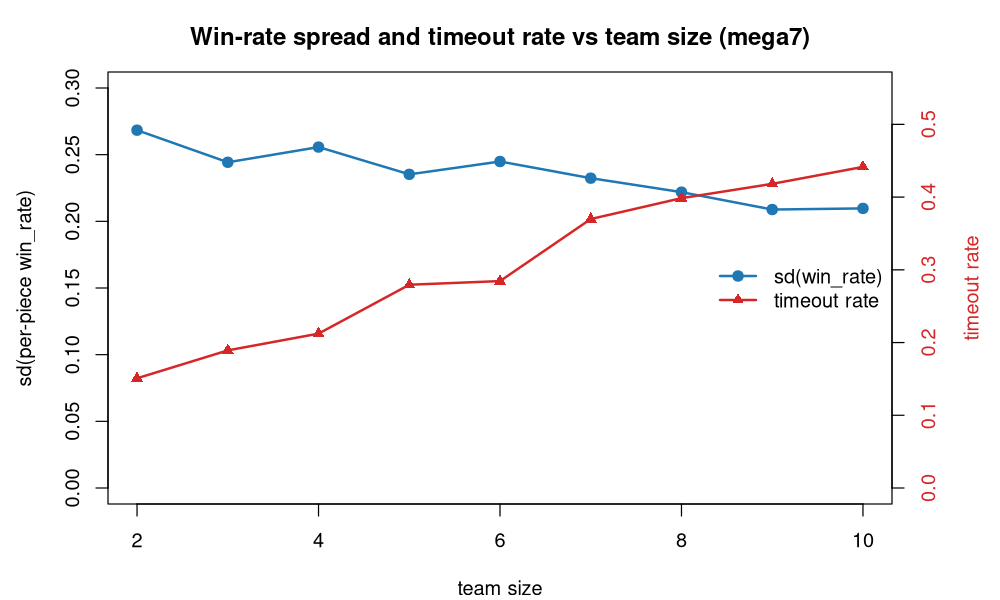
\includegraphics[width=0.86\linewidth,height=0.42\textheight,keepaspectratio]{plots/m7_02_variance_timeout_vs_size.png}
\caption*{\small win\textbackslash\{\}\_rate spread and timeout vs team size}
\end{figure}

\section*{3. Role balance}

\subsection*{3.1 Win rate by team size}

\begin{figure}[H]\centering
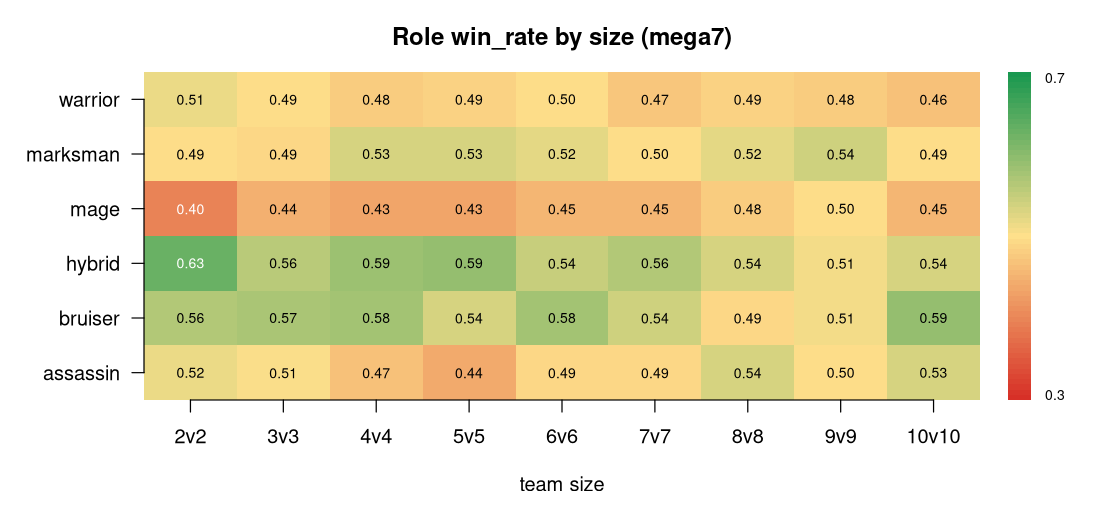
\includegraphics[width=0.86\linewidth,height=0.42\textheight,keepaspectratio]{plots/m7_04_role_wr_heatmap.png}
\caption*{\small Role win\textbackslash\{\}\_rate by size (heatmap)}
\end{figure}

Pooled (combined) role win rates:\\

\medskip
\begin{tabularx}{\linewidth}{Lr}
\toprule
\textbf{role} & \textbf{win\_rate} \\
\midrule
mage & 0.458 \\
warrior & 0.486 \\
assassin & 0.496 \\
marksman & 0.515 \\
bruiser & 0.546 \\
hybrid & 0.559 \\
\bottomrule
\end{tabularx}
\medskip

Mage is the floor at every size except 9v9. Hybrid and bruiser are the ceiling --- the same two outliers flagged in mega6.\\

\subsection*{3.2 Tuning residuals (wr\_delta)}

Pooled (combined) role \texttt{wr\_\allowbreak{}delta}:\\

\medskip
\begin{tabularx}{\linewidth}{LL}
\toprule
\textbf{role} & \textbf{wr\_delta} \\
\midrule
hybrid & −0.030 \\
mage & −0.018 \\
assassin & −0.001 \\
bruiser & +0.008 \\
warrior & +0.024 \\
marksman & +0.029 \\
\bottomrule
\end{tabularx}
\medskip

The story splits from raw win rate. **Hybrid is the most *under-budget* role\textbf{ despite the highest raw win rate --- its members are high-power T10 bosses that win on stats but under-deliver on kit. }Marksman and warrior over-deliver** (+0.025--0.029): they punch above their power budget. Mage is under on both raw and budget.\\

\begin{figure}[H]\centering
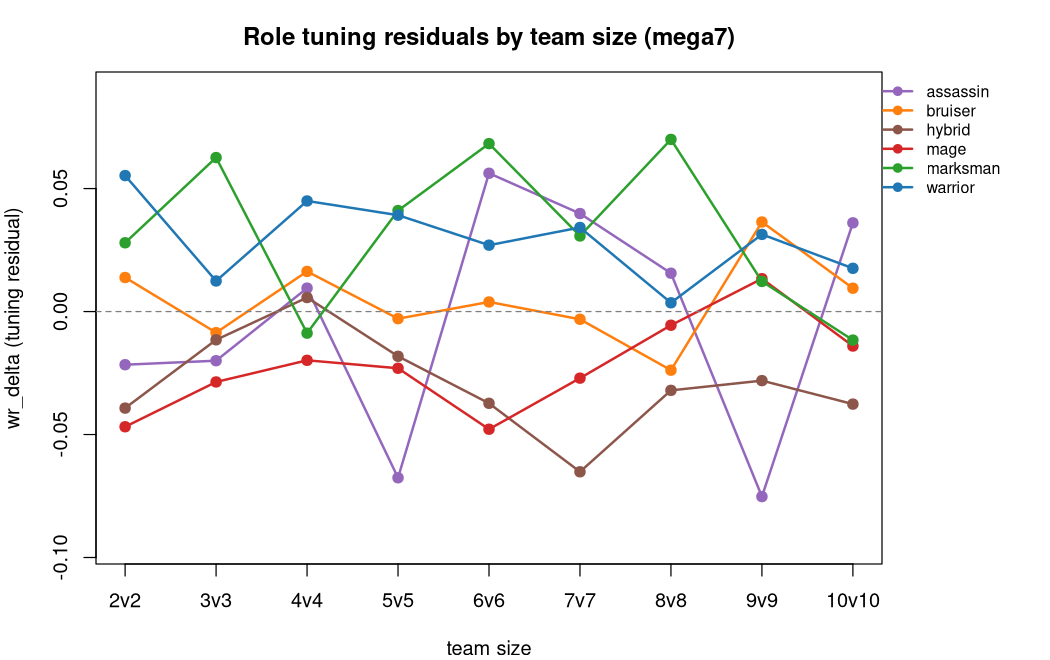
\includegraphics[width=0.86\linewidth,height=0.42\textheight,keepaspectratio]{plots/m7_01_role_wrdelta_vs_size.png}
\caption*{\small Role tuning residuals by team size}
\end{figure}

\section*{4. Mage deficit}

\medskip
\begin{tabularx}{\linewidth}{LrrLr}
\toprule
\textbf{stage} & \textbf{mage} & \textbf{nonmage} & \textbf{within\_tier\_def} & \textbf{cor(tier,wr)} \\
\midrule
2v2 & 0.398 & 0.542 & 0.079 & 0.383 \\
3v3 & 0.444 & 0.519 & 0.011 & 0.290 \\
4v4 & 0.434 & 0.519 & 0.019 & 0.322 \\
5v5 & 0.432 & 0.514 & 0.045 & 0.255 \\
6v6 & 0.454 & 0.521 & 0.034 & 0.154 \\
7v7 & 0.453 & 0.506 & −0.016 & 0.265 \\
8v8 & 0.480 & 0.511 & −0.013 & 0.204 \\
9v9 & 0.499 & 0.502 & −0.004 & 0.223 \\
10v10 & 0.452 & 0.510 & 0.023 & 0.223 \\
\bottomrule
\end{tabularx}
\medskip

The within-tier deficit is sharply concentrated at \textbf{2v2 (0.079)} and is gone or inverted by 7v7--8v8. Mages scale *into* relevance with team size --- they need allies to survive long enough to ramp. Versus mega6 at matched sizes the picture is mixed: 2v2 slightly worse (+0.013), but 3v3/7v7/8v8 notably better (−0.036 to −0.038).\\

\begin{figure}[H]\centering
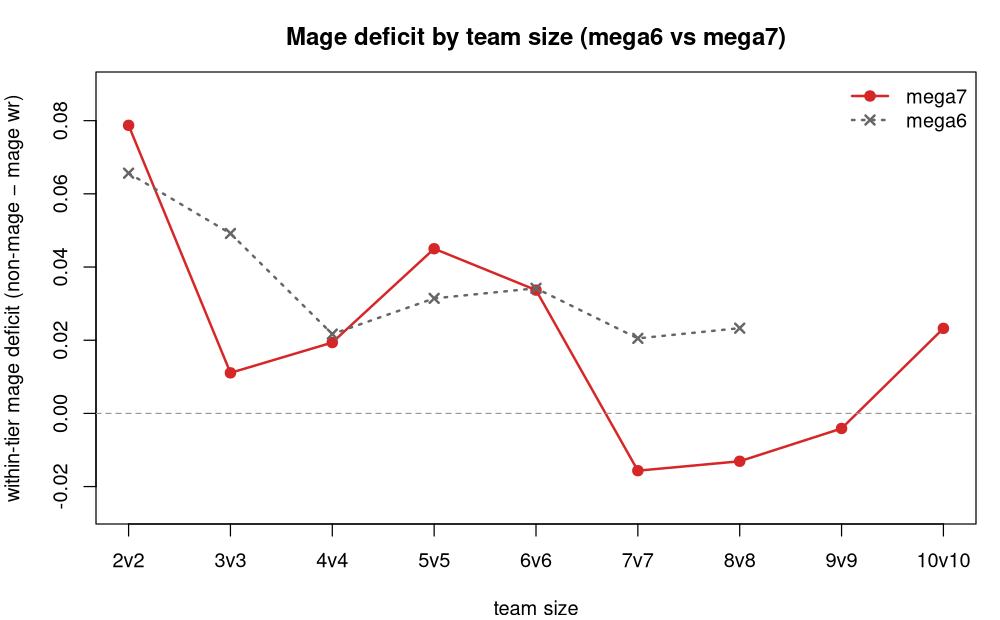
\includegraphics[width=0.86\linewidth,height=0.42\textheight,keepaspectratio]{plots/m7_03_mage_deficit_by_size.png}
\caption*{\small Mage deficit by team size: mega6 vs mega7}
\end{figure}

The worst individual mages (pooled \texttt{wr\_\allowbreak{}delta}) are \textbf{Hierarch} (clear T8 L3, −0.221), \textbf{Hoarfrost Owl} (snow T4 L3, −0.184), \textbf{Standard Bearer} (clear T3 L2, −0.179), \textbf{Fogveil Moth} (mist T5 L3, −0.170), \textbf{Drowned Siren} (rain T4 L1, −0.165). Note Hierarch --- it received the on-death barrier this session, which does nothing for its own survival; it remains the single most under-tuned mage. \textbf{Glade Heron L3 is on-budget (+0.022)} despite a 0.903 raw win rate (T8 L3 is *expected* to win that much) --- the rework landed in the right place.\\

\begin{figure}[H]\centering
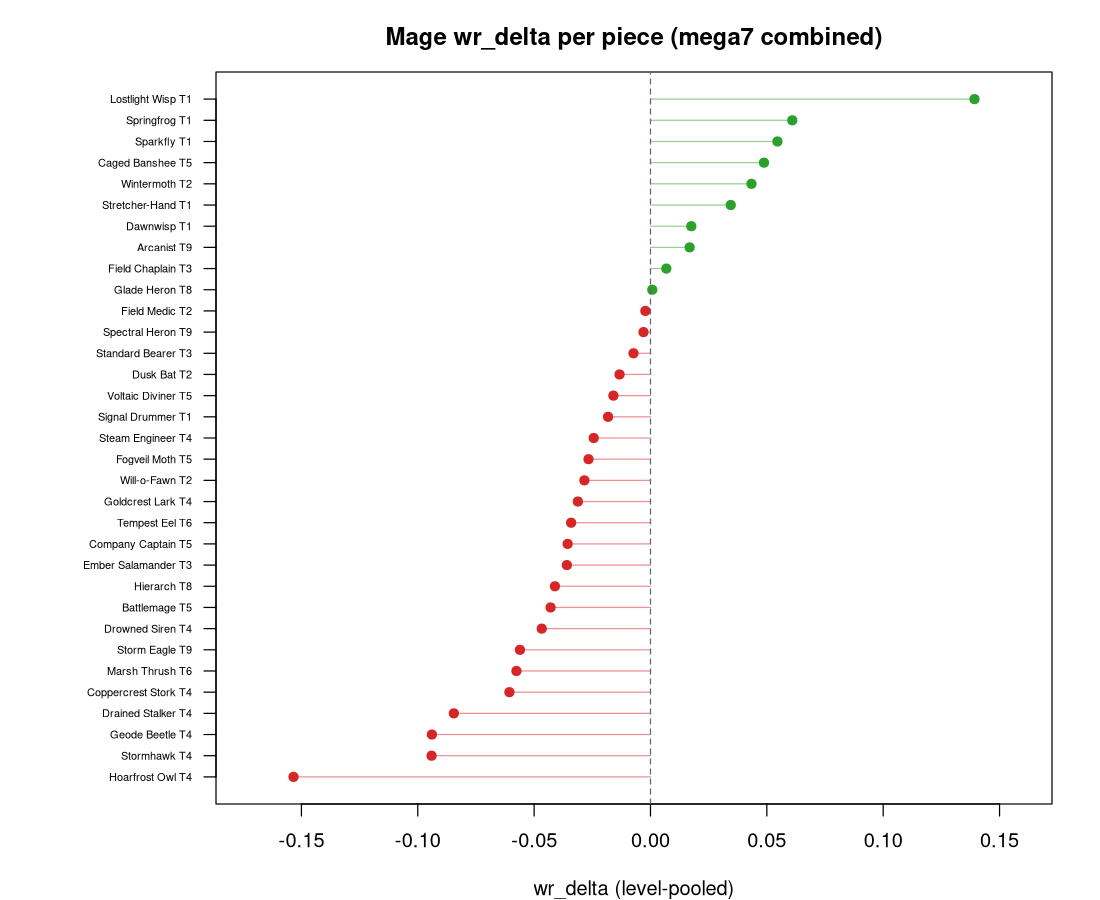
\includegraphics[width=0.86\linewidth,height=0.42\textheight,keepaspectratio]{plots/m7_08_mage_wrdelta.png}
\caption*{\small Mage wr\textbackslash\{\}\_delta per piece (combined)}
\end{figure}

\section*{5. Level effects}

\medskip
\begin{tabularx}{\linewidth}{rrLr}
\toprule
\textbf{level} & \textbf{win\_rate} & \textbf{wr\_delta} & \textbf{timeout} \\
\midrule
1 & 0.424 & +0.019 & 0.279 \\
2 & 0.480 & +0.004 & 0.277 \\
3 & 0.593 & −0.021 & 0.304 \\
\bottomrule
\end{tabularx}
\medskip

The level premium is steep (L1$\rightarrow$L3 = +0.17 raw) but \texttt{wr\_\allowbreak{}delta} stays small: L1 slightly under-delivers, L3 slightly over. Mixed-level teams will be L3-dominated, which is by design. No action needed.\\

\begin{figure}[H]\centering
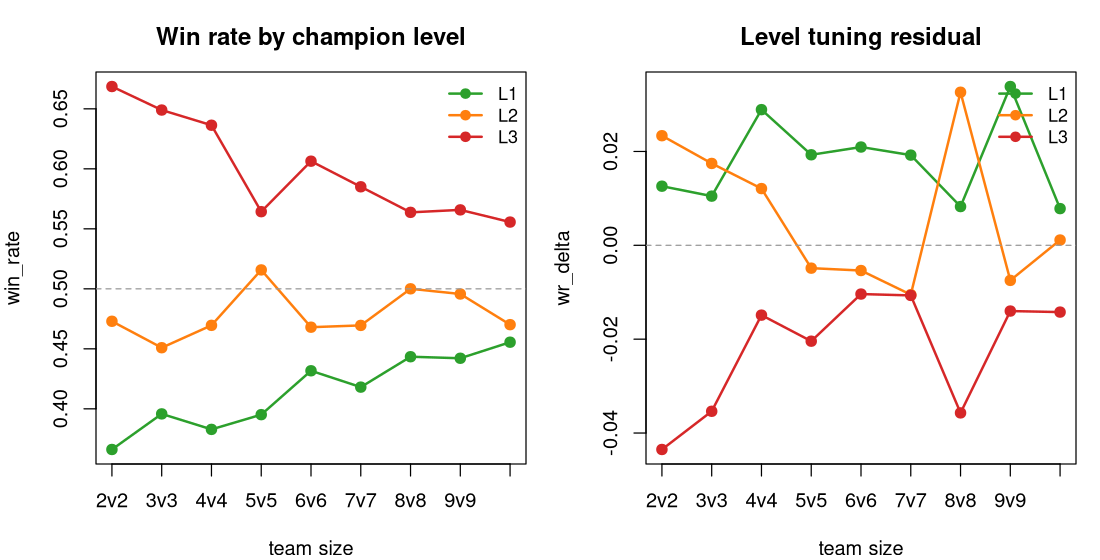
\includegraphics[width=0.86\linewidth,height=0.42\textheight,keepaspectratio]{plots/m7_05_level_effect.png}
\caption*{\small Win rate and tuning residual by champion level}
\end{figure}

\section*{6. Weather effects}

\textbf{Headline correction.} A first pass on this dataset reported a dominant \textbf{+0.18} own-vs-counter weather advantage. That number was wrong --- a metric artefact, not a balance fact. This section uses the corrected computation (raw per-weather win rates); the favor effect is real but \textbf{modest (\textasciitilde{}+0.01)}.\\

\textbf{The bug.} The \texttt{counter\_\allowbreak{}weather\_\allowbreak{}wr} column defaults to \textbf{0.0 when a piece has no games in its counter weather}. That conflates "no data" with "0\% win rate". It fires constantly: a piece's counter weather is one specific weather of six, and every \texttt{clear}-affinity piece has *no* counter weather at all (NEUTRAL on the ring). Result --- \texttt{counter\_\allowbreak{}weather\_\allowbreak{}wr == 0.\allowbreak{}0} in \textbf{37.1\%} of rows. Averaging those zeros in collapses the mean counter and manufactures a fake gap:\\

\medskip
\begin{tabularx}{\linewidth}{Lrrr}
\toprule
\textbf{computation} & \textbf{own} & \textbf{counter} & \textbf{own − counter} \\
\midrule
buggy column-average (zeros in) & 0.505 & 0.332 & +0.173 \\
\textbf{correct (raw per-weather win rate)} & \textbf{0.509} & \textbf{0.499} & \textbf{+0.010} \\
\bottomrule
\end{tabularx}
\medskip

Fixed in code: \texttt{weather\_\allowbreak{}metrics} now emits \texttt{NaN} (not \texttt{0.\allowbreak{}0}) for a weather the piece never played, and the CSV writer leaves the cell empty so aggregators skip it. This report recomputes from raw per-weather win rates and is unaffected.\\

\textbf{Corrected own-weather advantage by size} (own = win rate in own affinity weather; clear = no-favor baseline; counter = weather that preys on you):\\

\medskip
\begin{tabularx}{\linewidth}{Lrrrrr}
\toprule
\textbf{stage} & \textbf{clear (base)} & \textbf{own} & \textbf{counter} & \textbf{own − counter} & \textbf{own − clear} \\
\midrule
2v2 & 0.500 & 0.515 & 0.498 & +0.017 & +0.015 \\
4v4 & 0.500 & 0.505 & 0.498 & +0.007 & +0.005 \\
6v6 & 0.500 & 0.507 & 0.495 & +0.012 & +0.007 \\
8v8 & 0.500 & 0.508 & 0.499 & +0.009 & +0.008 \\
10v10 & 0.500 & 0.506 & 0.503 & +0.003 & +0.006 \\
\bottomrule
\end{tabularx}
\medskip

\textbf{Corrected per-affinity} (raw, pooled all stages):\\

\medskip
\begin{tabularx}{\linewidth}{Lrrrrr}
\toprule
\textbf{affinity} & \textbf{clear} & \textbf{own} & \textbf{counter} & \textbf{own − clear} & \textbf{own − counter} \\
\midrule
mist & 0.512 & 0.513 & 0.498 & +0.002 & +0.016 \\
cloudy & 0.506 & 0.530 & 0.494 & +0.025 & +0.037 \\
rain & 0.515 & 0.530 & 0.515 & +0.016 & +0.016 \\
snow & 0.509 & 0.516 & 0.495 & +0.007 & +0.022 \\
thunder & 0.491 & 0.511 & 0.496 & +0.020 & +0.015 \\
\bottomrule
\end{tabularx}
\medskip

Every affinity gains in its own weather and loses (or is flat) in its counter weather --- \textbf{the favor system works as designed, and the earlier snow/thunder "inversion" was thin-slice noise}, not a real effect. The magnitude is small (single-digit win-rate points), so weather favor is a flavour-and-edge system, *not* a dominant axis --- it does not overshadow kit or role. Whether $\pm$0.30 favor magnitude should produce a *larger* effect than this is a separate design question, but it is not overpowered.\\

\begin{figure}[H]\centering
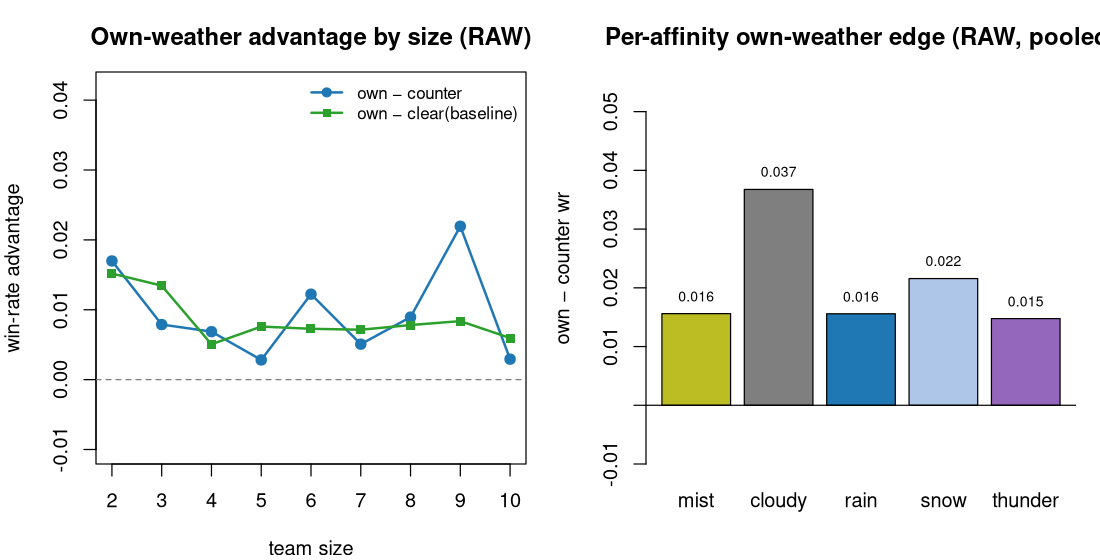
\includegraphics[width=0.86\linewidth,height=0.42\textheight,keepaspectratio]{plots/m7_06_weather_effects.png}
\caption*{\small Weather: corrected own-advantage by size and per-affinity edge}
\end{figure}

\section*{7. Timeouts}

\medskip
\begin{tabularx}{\linewidth}{Lrrrr}
\toprule
\textbf{role} & \textbf{2v2} & \textbf{5v5} & \textbf{8v8} & \textbf{10v10} \\
\midrule
assassin & 0.131 & 0.312 & 0.352 & 0.483 \\
bruiser & 0.320 & 0.378 & 0.508 & 0.398 \\
hybrid & 0.120 & 0.289 & 0.350 & 0.405 \\
mage & 0.160 & 0.248 & 0.406 & 0.448 \\
marksman & 0.078 & 0.257 & 0.379 & 0.404 \\
warrior & 0.145 & 0.271 & 0.412 & 0.469 \\
\bottomrule
\end{tabularx}
\medskip

Bruisers stall hardest at small/mid sizes (high survivability, low burst), consistent with mega6. At the largest sizes nearly half of all battles time out --- the 12,000-tick cap is too tight for 10v10 to resolve organically. Large-format role reads should be treated cautiously because of this.\\

\section*{8. Outliers and tuning priorities}

\subsection*{8.1 How odd are the residuals? Distribution shape}

Before naming individual pieces, the question "how odd are these \texttt{wr\_\allowbreak{}delta}s" is best answered by the *shape* of the pooled-residual distribution. The boxplots below break \texttt{wr\_\allowbreak{}delta} out by role and by tier; the histogram/Q-Q pair shows the overall distribution against a normal reference.\\

\begin{figure}[H]\centering
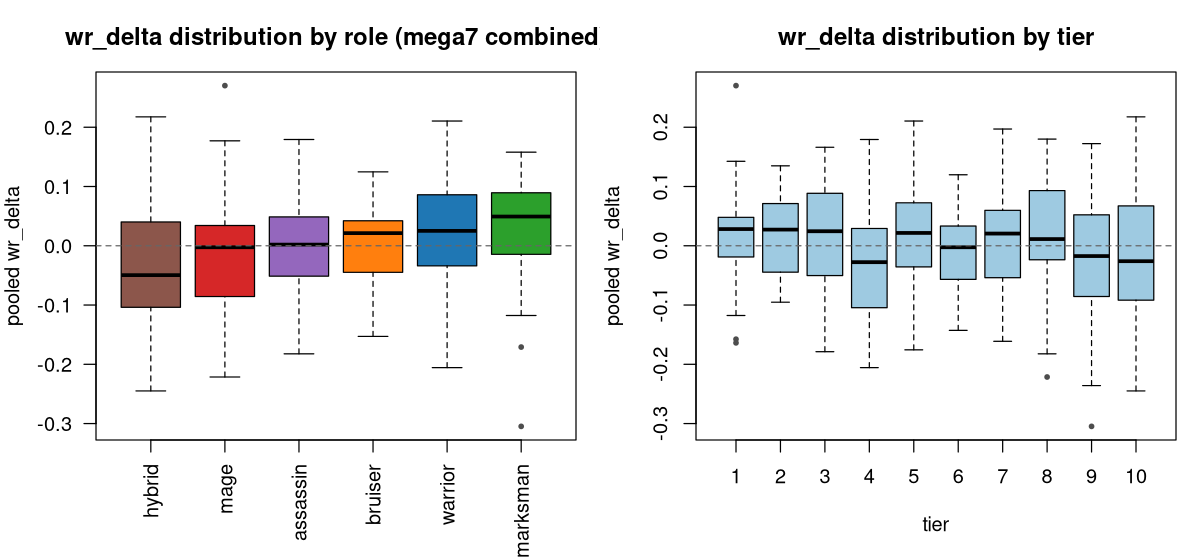
\includegraphics[width=0.86\linewidth,height=0.42\textheight,keepaspectratio]{plots/m7_09_wrdelta_boxplots.png}
\caption*{\small wr\textbackslash\{\}\_delta distribution by role and by tier (boxplots)}
\end{figure}

\begin{figure}[H]\centering
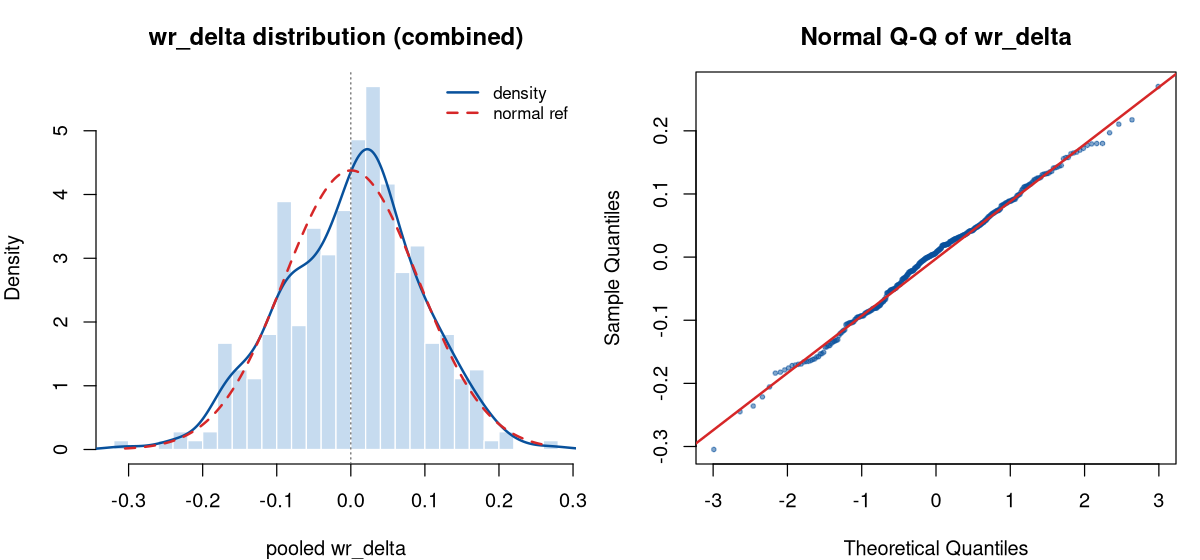
\includegraphics[width=0.86\linewidth,height=0.42\textheight,keepaspectratio]{plots/m7_10_wrdelta_distribution.png}
\caption*{\small wr\textbackslash\{\}\_delta distribution: histogram + density vs normal, and normal Q-Q}
\end{figure}

The pooled \texttt{wr\_\allowbreak{}delta} distribution is \textbf{near-normal in the body and only mildly heavy-tailed} (Q-Q is straight from roughly −2σ to +2σ, with a handful of points pulling away at each end). Practically: the residuals are *not* pathologically wild --- most pieces sit within $\pm$0.10 of budget, and the named outliers below are genuine tail events (|z| ≳ 2 within their tier), not an artefact of a fat-tailed mess. By role, \textbf{hybrid and mage carry the most negative-skewed boxes} (medians below 0, long lower whiskers); \textbf{warrior and marksman skew positive}. By tier the spread is fairly uniform --- high tiers are *not* systematically noisier once pooled --- which is what justifies the within-tier z-score below.\\

\subsection*{8.2 Absolute outliers (largest |wr\_delta|)}

\texttt{wd\_\allowbreak{}z} = within-tier z-score of \texttt{wr\_\allowbreak{}delta} (how many SD from the piece's *tier cohort* mean). |z| ≳ 2 $\approx$ a genuine per-tier outlier, not tier-position noise.\\

\begin{figure}[H]\centering
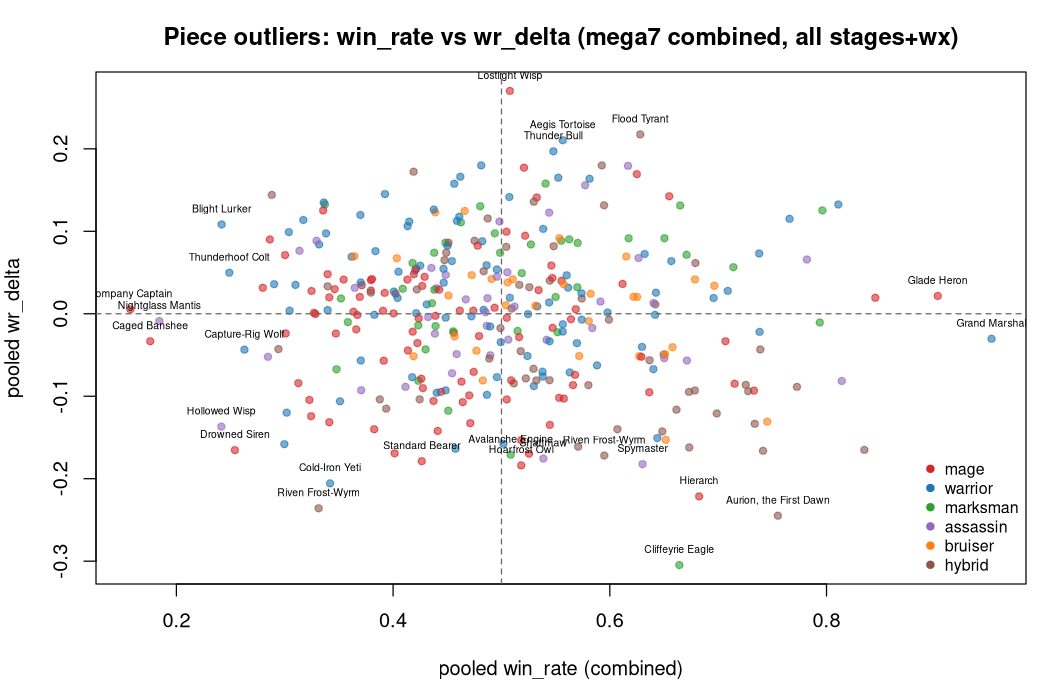
\includegraphics[width=0.86\linewidth,height=0.42\textheight,keepaspectratio]{plots/m7_07_outlier_scatter.png}
\caption*{\small Piece outliers: win\textbackslash\{\}\_rate vs wr\textbackslash\{\}\_delta (combined)}
\end{figure}

\textbf{Most under-tuned (pooled \texttt{wr\_\allowbreak{}delta}):}\\

\medskip
\begin{tabularx}{\linewidth}{LLLrrrLL}
\toprule
\textbf{name} & \textbf{affinity} & \textbf{role} & \textbf{tier} & \textbf{level} & \textbf{win\_rate} & \textbf{wr\_delta} & \textbf{wd\_z} \\
\midrule
Cliffeyrie Eagle & cloudy & marksman & 9 & 3 & 0.664 & −0.305 & −2.76 \\
Aurion, the First Dawn & clear & hybrid & 10 & 3 & 0.755 & −0.245 & −2.21 \\
Riven Frost-Wyrm & snow & hybrid & 9 & 1 & 0.331 & −0.236 & −2.10 \\
Hierarch & clear & mage & 8 & 3 & 0.682 & −0.221 & −2.35 \\
Cold-Iron Yeti & snow & warrior & 4 & 2 & 0.342 & −0.206 & −1.87 \\
Hoarfrost Owl & snow & mage & 4 & 3 & 0.518 & −0.184 & −1.64 \\
Spymaster & clear & assassin & 8 & 3 & 0.630 & −0.182 & −1.96 \\
Standard Bearer & clear & mage & 3 & 2 & 0.426 & −0.179 & −2.19 \\
Shaftmaw & cloudy & assassin & 5 & 2 & 0.539 & −0.176 & −1.96 \\
Avalanche Engine & snow & marksman & 5 & 2 & 0.508 & −0.171 & −1.91 \\
Fogveil Moth & mist & mage & 5 & 3 & 0.525 & −0.170 & −1.90 \\
Umbra, the Mountain's Shadow & cloudy & hybrid & 10 & 3 & 0.741 & −0.166 & −1.45 \\
Drowned Siren & rain & mage & 4 & 1 & 0.254 & −0.165 & −1.44 \\
\bottomrule
\end{tabularx}
\medskip

\textbf{Most over-tuned:}\\

\medskip
\begin{tabularx}{\linewidth}{LLLrrrrr}
\toprule
\textbf{name} & \textbf{affinity} & \textbf{role} & \textbf{tier} & \textbf{level} & \textbf{win\_rate} & \textbf{wr\_delta} & \textbf{wd\_z} \\
\midrule
Lostlight Wisp & mist & mage & 1 & 1 & 0.508 & +0.270 & +2.89 \\
Flood Tyrant & rain & hybrid & 10 & 2 & 0.628 & +0.217 & +2.25 \\
Aegis Tortoise & clear & warrior & 5 & 3 & 0.557 & +0.210 & +2.05 \\
Thunder Bull & thunder & warrior & 7 & 2 & 0.548 & +0.197 & +2.20 \\
Storm Tyrant & thunder & hybrid & 10 & 2 & 0.593 & +0.180 & +1.88 \\
Frostfang Wolverine & snow & warrior & 8 & 1 & 0.481 & +0.180 & +1.67 \\
Hollow Elk & mist & assassin & 4 & 3 & 0.617 & +0.179 & +2.23 \\
Caged Banshee & mist & mage & 5 & 3 & 0.521 & +0.177 & +1.70 \\
Sundered Lord & mist & hybrid & 9 & 1 & 0.419 & +0.172 & +1.84 \\
Voltaic Diviner & thunder & mage & 5 & 2 & 0.625 & +0.169 & +1.62 \\
Heavy Knight & clear & warrior & 4 & 2 & 0.581 & +0.164 & +2.07 \\
Iron-Collared Hound & snow & warrior & 3 & 3 & 0.462 & +0.166 & +1.70 \\
Cannoneer & clear & marksman & 8 & 1 & 0.541 & +0.158 & +1.45 \\
\bottomrule
\end{tabularx}
\medskip

The under-tuned list is dominated by \textbf{high-tier hybrids/mages that win on raw power but miss their budget} (Aurion, Umbra, Hierarch) and \textbf{snow pieces} (Riven Frost-Wyrm, Cold-Iron Yeti, Hoarfrost Owl, Avalanche Engine) --- reinforcing the snow-affinity anomaly from \S{}6. The over-tuned list is led by a T1 mage (Lostlight Wisp, z=+2.9 --- the single oddest piece in the sweep) and the rain/thunder hybrid Tyrants. Full 30-row absolute-outlier table: \texttt{tables/\allowbreak{}m7\_\allowbreak{}abs\_\allowbreak{}outliers.\allowbreak{}csv}.\\

\subsection*{8.3 Spread outliers --- context-volatility of wr\_delta}

A piece can also be "odd" by being \textbf{inconsistent}: a pooled \texttt{wr\_\allowbreak{}delta} near 0 that hides large swings across formats/weathers is as much a balance concern as a flat large residual. Per-(stage,weather) cells are thin here (often 1--2 matches), so raw spread is dominated by binomial noise. We compute each piece's match-weighted \texttt{sd(\allowbreak{}wr\_\allowbreak{}delta)\allowbreak{}} across its 54 contexts, subtract the \textbf{expected binomial-noise sd} (estimated from the piece's pooled win-rate, *not* per-cell --- a per-cell estimate collapses to 0 on single-match cells and fabricates spread), and rank by the \textbf{excess}.\\

\begin{figure}[H]\centering
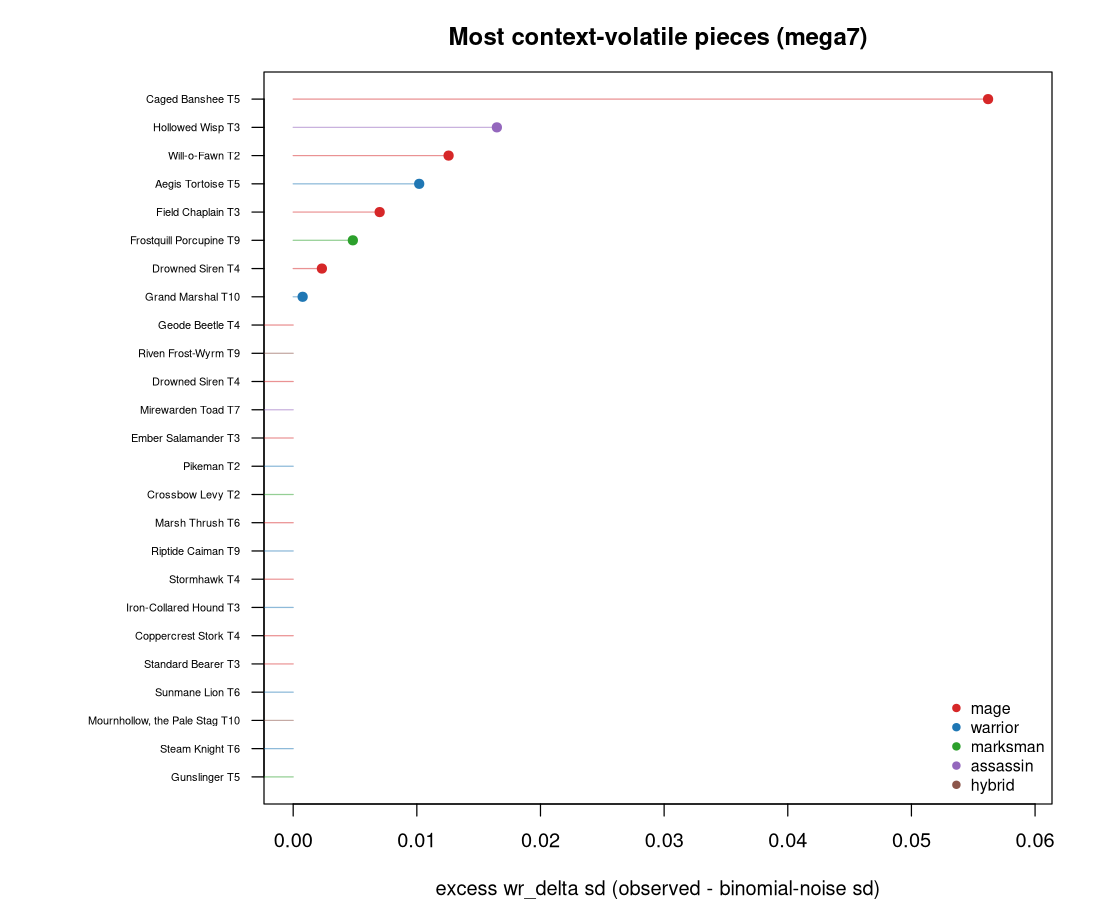
\includegraphics[width=0.86\linewidth,height=0.42\textheight,keepaspectratio]{plots/m7_11_spread_outliers.png}
\caption*{\small Most context-volatile pieces (excess wr\textbackslash\{\}\_delta sd beyond noise)}
\end{figure}

\textbf{Key result: spread is almost entirely sampling noise.} Only \textbf{8 of 360} pieces show \texttt{excess\_\allowbreak{}sd > 0} --- i.e. for \textasciitilde{}98\% of pieces, the observed across-context \texttt{wr\_\allowbreak{}delta} spread is fully explained by thin-sample binomial noise. The genuine context-volatile pieces:\\

\medskip
\begin{tabularx}{\linewidth}{LLLrrLrrr}
\toprule
\textbf{name} & \textbf{affinity} & \textbf{role} & \textbf{tier} & \textbf{tot\_matches} & \textbf{wd\_pooled} & \textbf{wd\_sd} & \textbf{noise\_sd} & \textbf{excess\_sd} \\
\midrule
Caged Banshee & mist & mage & 5 & 60 & +0.050 & 0.540 & 0.483 & +0.056 \\
Hollowed Wisp & mist & assassin & 3 & 156 & −0.144 & 0.261 & 0.244 & +0.016 \\
Will-o-Fawn & mist & mage & 2 & 330 & −0.038 & 0.225 & 0.212 & +0.013 \\
Aegis Tortoise & clear & warrior & 5 & 84 & +0.143 & 0.401 & 0.391 & +0.010 \\
Field Chaplain & clear & mage & 3 & 390 & −0.055 & 0.197 & 0.190 & +0.007 \\
Frostquill Porcupine & snow & marksman & 9 & 312 & +0.013 & 0.163 & 0.158 & +0.005 \\
Drowned Siren & rain & mage & 4 & 192 & +0.230 & 0.231 & 0.228 & +0.002 \\
Grand Marshal & clear & warrior & 10 & 198 & −0.015 & 0.117 & 0.116 & +0.001 \\
\bottomrule
\end{tabularx}
\medskip

The excesses are \textbf{small in absolute terms} ($\leq$0.056) and the leaders are thin-sample (\texttt{tot\_\allowbreak{}matches} 60--390). Three of the eight are \textbf{mist} pieces --- mist is the affinity whose counter-relationship gets sampled least evenly, so a residual mist-driven swing is plausible but unconfirmed at this depth. \textbf{Takeaway:} \texttt{wr\_\allowbreak{}delta} is not meaningfully context-volatile in mega7 once noise is removed --- the outliers worth acting on are the *absolute* ones in \S{}8.2, not spread. Full table: \texttt{tables/\allowbreak{}m7\_\allowbreak{}spread\_\allowbreak{}outliers.\allowbreak{}csv}. To confirm any spread finding, re-run with \texttt{-\allowbreak{}-\allowbreak{}total-\allowbreak{}battles} raised \textasciitilde{}5--10$\times$ so per-cell depth lifts above the binomial-noise floor.\\

\section*{9. Recommendations}

\begin{itemize}
\item \textbf{Mage early-game power (priority).} Target the 2v2 within-tier deficit specifically --- it vanishes at scale, so the fix is early survivability/damage, not late-game. Worst offenders: Hierarch, Hoarfrost Owl, Standard Bearer, Fogveil Moth, Drowned Siren.
\item \textbf{T10 hybrid boss kits (Aurion, Aerion, Storm Tyrant) under-deliver vs budget} --- recurring since mega6. Their kits need a pass; they should top the chart, not merely win on raw power.
\item \textbf{Hierarch.} Most under-tuned mage; the new on-death barrier helps allies, not itself. Needs a personal-survivability or damage buff.
\item \textbf{Weather favor: no action needed.} Corrected analysis (\S{}6) shows it working as designed at a modest \textasciitilde{}+0.01 edge. If a *stronger* competitive weather effect is wanted, the $\pm$0.30 magnitude could be revisited --- but it is not a balance problem. The metric bug that overstated it has been fixed in \texttt{weather\_\allowbreak{}metrics}.
\item \textbf{Validated this session:} Glade Heron L3 is on-budget (+0.022); the poison percentage-decay model produced no runaway poison outliers in team play.
\end{itemize}

\section*{10. Reproducibility}

\begin{lstlisting}
# 1. Run the sweep (current working tree)
python -m tools.simulation.mega --total-battles <N> --skip 1v1 \
    --workers 16 --out results/mega/mega7

# 2. Analysis + tables + cache
Rscript reviews/mega_sim/11_mega7.R

# 3. Figures
Rscript reviews/mega_sim/12_mega7_plots.R

# 4. This PDF
python3 reviews/mega_sim/build_mega7_pdf.py
\end{lstlisting}

Tables written to \texttt{reviews/\allowbreak{}mega\_\allowbreak{}sim/\allowbreak{}tables/\allowbreak{}m7\_\allowbreak{}*.\allowbreak{}csv}; cache to \texttt{cache\_\allowbreak{}mega7.\allowbreak{}rds}; figures to \texttt{reviews/\allowbreak{}mega\_\allowbreak{}sim/\allowbreak{}plots/\allowbreak{}m7\_\allowbreak{}*.\allowbreak{}png}. The engine is byte-deterministic --- same tree + same flags reproduce the CSVs exactly.\\

\end{document}